\anexo{Fluxograma de Integralização Curricular}
\label{an:fluxograma}

\begin{center}
\resizebox{.75\textwidth}{!}{\rotatebox{90}{%
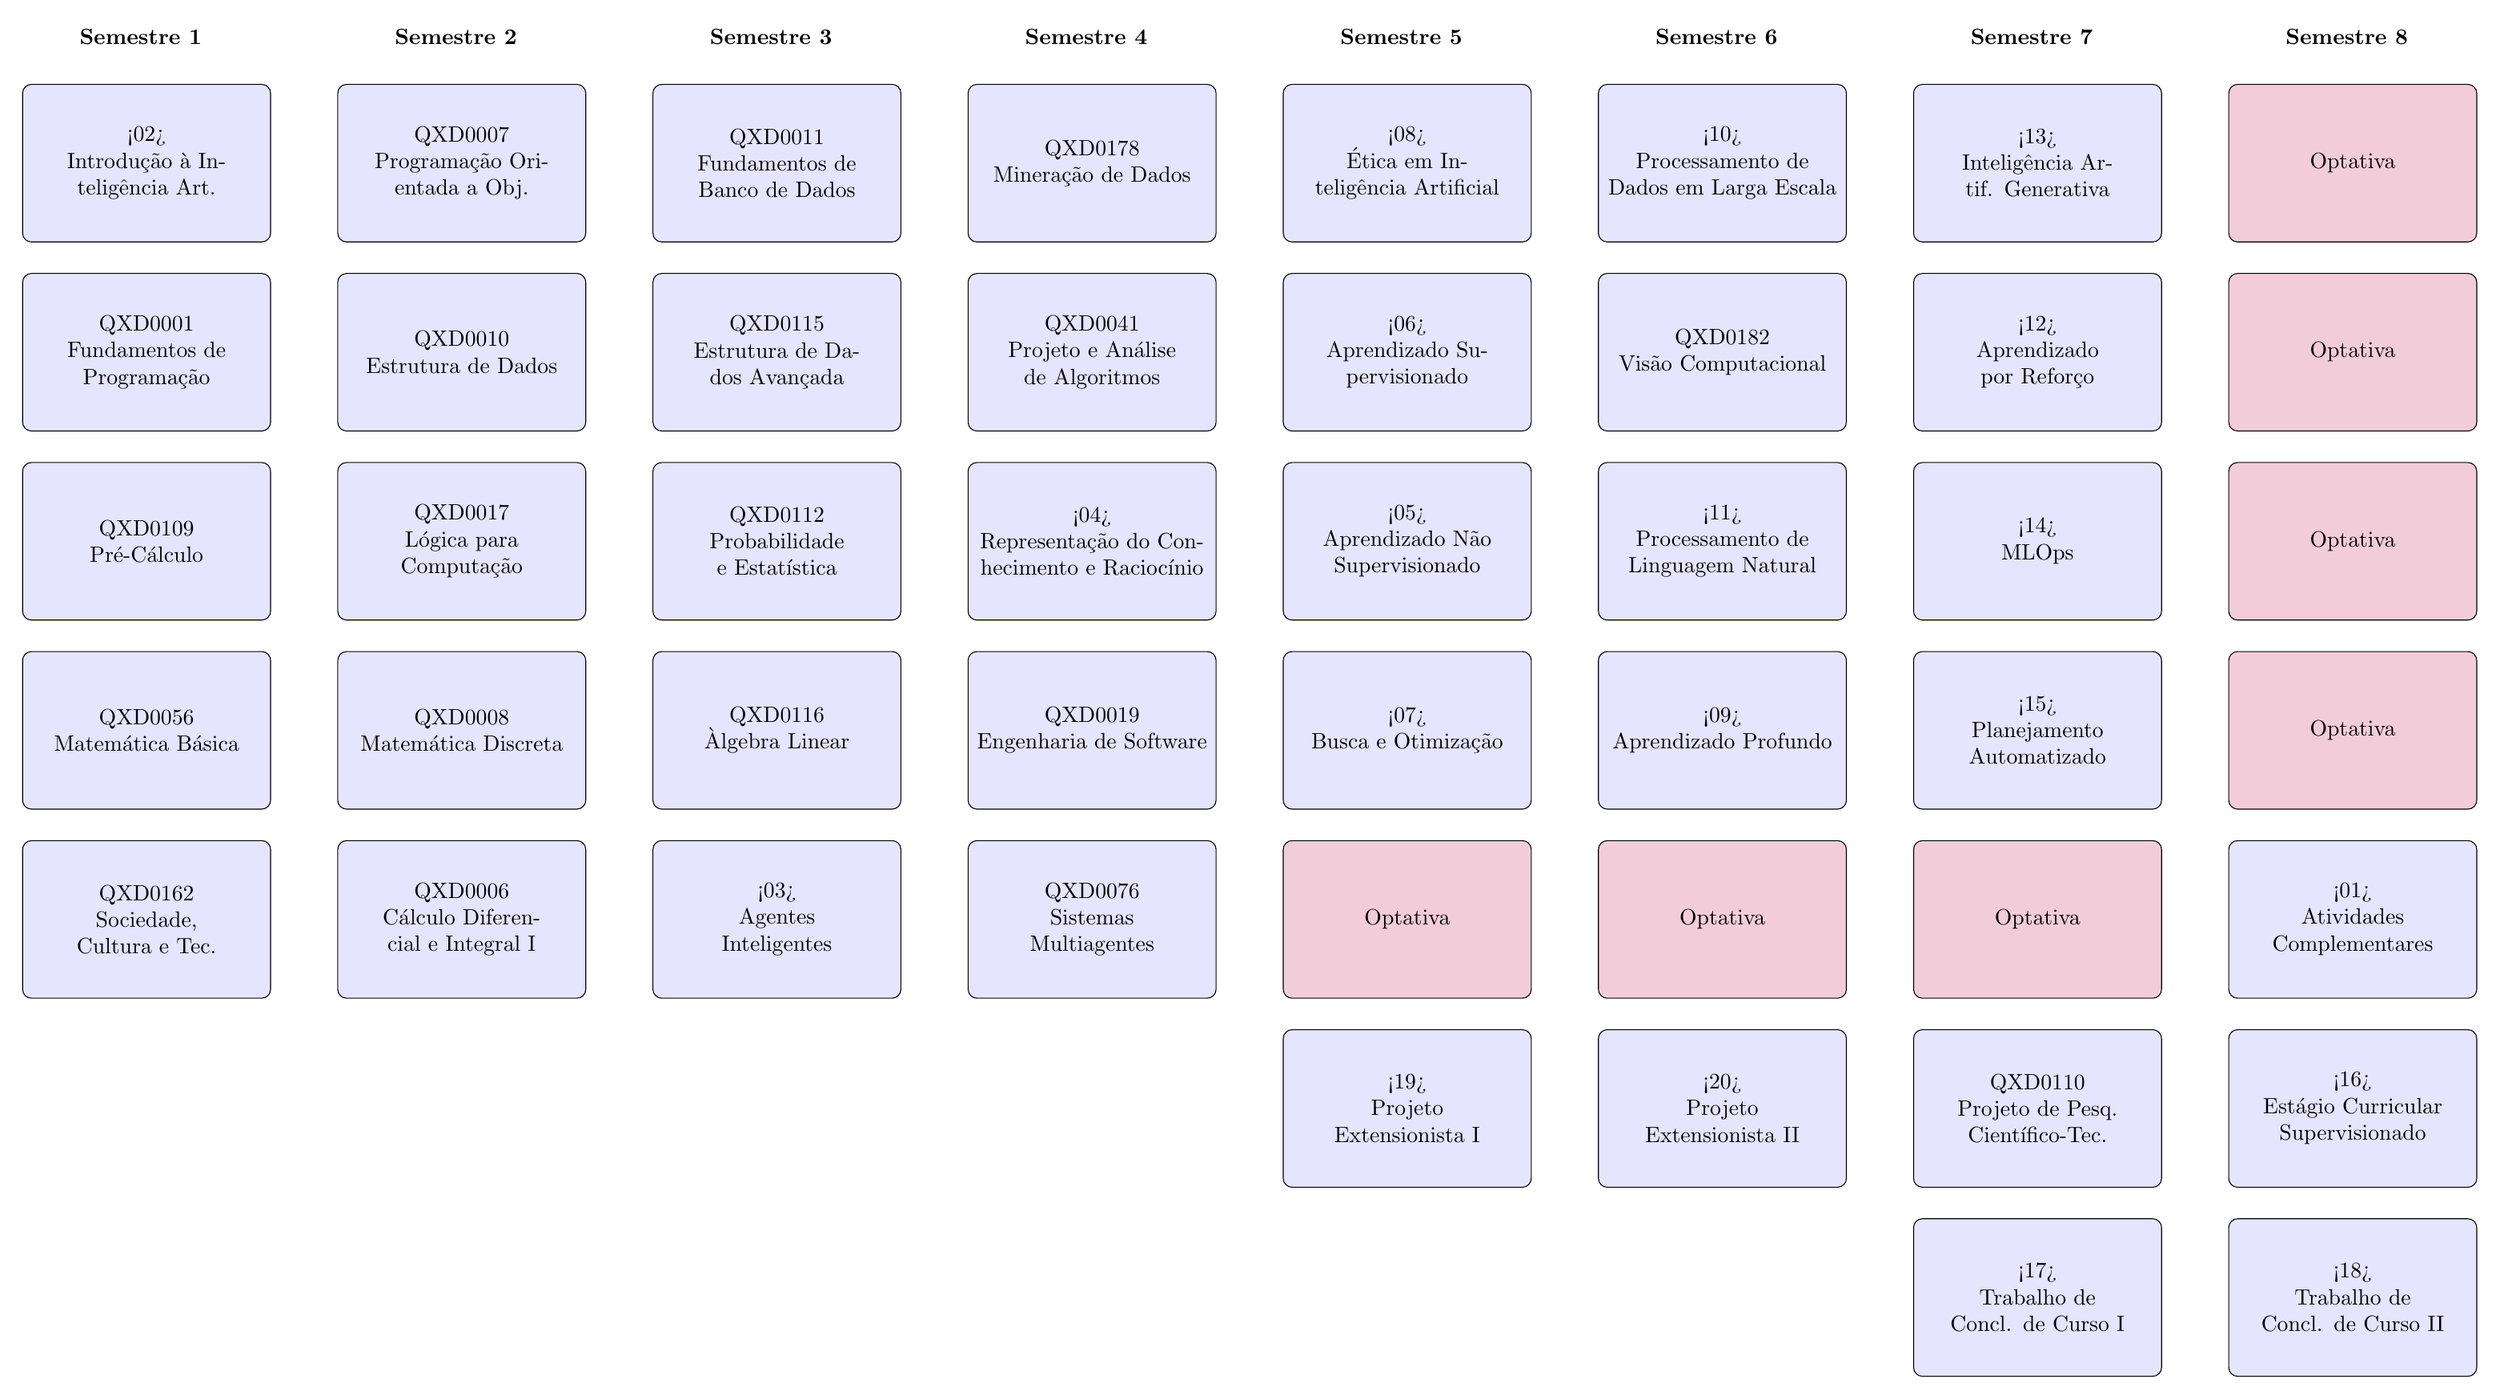
\begin{tikzpicture}[
  node distance=0.6cm and 1.5cm,
  box/.style={draw, rounded corners, fill=blue!10, text width=3.7cm, minimum height=2.5cm, align=center},
  opt/.style={draw, rounded corners, fill=purple!20, text width=3.7cm, minimum height=2.5cm, align=center},
  label/.style={font=\bfseries, anchor=east}]

% Labels dos semestres
\node[label] at ( 1, 2) {Semestre 1};
\node[label] at ( 6, 2) {Semestre 2};
\node[label] at (11,2) {Semestre 3};
\node[label] at (16,2) {Semestre 4};
\node[label] at (21,2) {Semestre 5};
\node[label] at (26,2) {Semestre 6};
\node[label] at (31,2) {Semestre 7};
\node[label] at (36,2) {Semestre 8};

% Disciplinas (linha a linha)
% Linha 1
\node[box] at ( 0, 0) {<02> \\ Introdu\c{c}\~ao \`a Intelig\^encia Art.};
\node[box] at ( 5, 0) {QXD0007 \\ Programa\c{c}\~ao Orientada a Obj.};
\node[box] at (10, 0) {QXD0011 \\ Fundamentos de Banco de Dados};
\node[box] at (15, 0) {QXD0178 \\ Minera\c{c}\~ao de Dados};
\node[box] at (20, 0) {<08> \\ \'{E}tica em Inteligência Artificial};
\node[box] at (25, 0) {<10> \\ Processamento de Dados em Larga Escala};
\node[box] at (30, 0) {<13> \\ Intelig\^encia Artif. Generativa};
\node[opt] at (35, 0) {Optativa};

% Linha 2
\node[box] at ( 0, -3) {QXD0001 \\ Fundamentos de Programa\c{c}\~ao};
\node[box] at ( 5, -3) {QXD0010 \\ Estrutura de Dados};
\node[box] at (10, -3) {QXD0115 \\ Estrutura de Dados Avan\c{c}ada};
\node[box] at (15, -3) {QXD0041 \\ Projeto e An\'alise de Algoritmos};
\node[box] at (20, -3) {<06> \\ Aprendizado Supervisionado};
\node[box] at (25, -3) {QXD0182 \\ Vis\~ao Computacional};
\node[box] at (30, -3) {<12> \\ Aprendizado por Refor\c{c}o};
\node[opt] at (35, -3) {Optativa};

% Linha 3
\node[box] at ( 0, -6) {QXD0109 \\ Pr\'e-C\'alculo};
\node[box] at ( 5, -6) {QXD0017 \\ L\'ogica para Computa\c{c}\~ao};
\node[box] at (10, -6) {QXD0112 \\ Probabilidade e Estat\'istica};
\node[box] at (15, -6) {<04> \\ Representação do Conhecimento e Racioc\'inio};
\node[box] at (20, -6) {<05> \\ Aprendizado N\~ao Supervisionado};
\node[box] at (25, -6) {<11> \\ Processamento de Linguagem Natural};
\node[box] at (30, -6) {<14> \\ MLOps};
\node[opt] at (35, -6) {Optativa};

% Linha 4
\node[box] at ( 0, -9) {QXD0056 \\ Matem\'atica B\'asica};
\node[box] at ( 5, -9) {QXD0008 \\ Matem\'atica Discreta};
\node[box] at (10, -9) {QXD0116 \\ \`Algebra Linear};
\node[box] at (15, -9) {QXD0019 \\ Engenharia de Software};
\node[box] at (20, -9) {<07> \\ Busca e Otimiza\c{c}\~ao};
\node[box] at (25, -9) {<09> \\ Aprendizado Profundo};
\node[box] at (30, -9) {<15> \\ Planejamento Automatizado};
\node[opt] at (35, -9) {Optativa};

% Linha 5
\node[box] at ( 0, -12) {QXD0162 \\ Sociedade,\\Cultura e Tec.};
\node[box] at ( 5, -12) {QXD0006 \\ C\'alculo Diferencial e Integral I};
\node[box] at (10, -12) {<03> \\ Agentes\\Inteligentes};
\node[box] at (15, -12) {QXD0076 \\ Sistemas\\Multiagentes};
\node[opt] at (20, -12) {Optativa};
\node[opt] at (25, -12) {Optativa};
\node[opt] at (30, -12) {Optativa};
\node[box] at (35, -12) {<01> \\ Atividades \\ Complementares};

% Linha 6
\node[box] at (20, -15) {<19> \\ Projeto\\Extensionista I};
\node[box] at (25, -15) {<20> \\ Projeto\\Extensionista II};
\node[box] at (30, -15) {QXD0110 \\ Projeto de Pesq. Científico-Tec.};
\node[box] at (35, -15) {<16> \\ Est\'agio Curricular \\ Supervisionado};

% Linha 7
\node[box] at (30, -18) {<17> \\ Trabalho de\\Concl. de Curso I};
\node[box] at (35, -18) {<18> \\ Trabalho de\\Concl. de Curso II};

\end{tikzpicture}
}}
\end{center}

